%
% Template Laporan Skripsi/Thesis 
%
% @author  Andreas Febrian, Lia Sadita 
% @version 1.03
%
% Dokumen ini dibuat berdasarkan standar IEEE dalam membuat class untuk 
% LaTeX dan konfigurasi LaTeX yang digunakan Fahrurrozi Rahman ketika 
% membuat laporan skripsi. Konfigurasi yang lama telah disesuaikan dengan 
% aturan penulisan thesis yang dikeluarkan UI pada tahun 2008.
%

%
% Tipe dokumen adalah report dengan satu kolom. 
%
\documentclass[12pt, a4paper, onecolumn, oneside, final]{report}

% Load konfigurasi LaTeX untuk tipe laporan thesis
\usepackage{uithesis}


% Load konfigurasi khusus untuk laporan yang sedang dibuat
%-----------------------------------------------------------------------------%
% Informasi Mengenai Dokumen
%-----------------------------------------------------------------------------%
% 
% Judul laporan. 
\var{\judul}{PR 3 Pemrograman di Lingkungan GPU}
% 
% Tulis kembali judul laporan, kali ini akan diubah menjadi huruf kapital
\Var{\Judul}{PR 3 Pemrograman di Lingkungan GPU}
% 
% Tulis kembali judul laporan namun dengan bahasa Ingris
%\var{\judulInggris}{Unknown Title for Final Report/Thesis/Disertation}

% 
% Tipe laporan, dapat berisi Skripsi, Tugas Akhir, Thesis, atau Disertasi
\var{\type}{Laporan Tugas Pemrograman Paralel}
% 
% Tulis kembali tipe laporan, kali ini akan diubah menjadi huruf kapital
\Var{\Type}{Laporan Tugas Pemrograman Paralel}
% 
% Tulis nama penulis 
\var{\penulis}{Kelompok III}
% 
% Tulis kembali nama penulis, kali ini akan diubah menjadi huruf kapital
\Var{\Penulis}{Kelompok III}
% 
% Tulis NPM penulis
\var{\npm}{XXXXXXXXXX}

\var{\npmPertama}{1506706276}
\var{\npmKedua}{1506706295}
\var{\npmKetiga}{1506706345}

\var{\namaPertama}{Muhammad Fathurachman}
\var{\namaKedua}{Otniel Yosi Viktorisa}
\var{\namaKetiga}{Yohanes Gultom}

% 
% Tuliskan Fakultas dimana penulis berada
\Var{\Fakultas}{Ilmu Komputer}
\var{\fakultas}{Ilmu Komputer}
% 
% Tuliskan Program Studi yang diambil penulis
\Var{\Program}{Magister Ilmu Komputer}
\var{\program}{Magister Ilmu Komputer}
% 
% Tuliskan tahun publikasi laporan
\Var{\bulanTahun}{Mei 2016}
% 
% Tuliskan gelar yang akan diperoleh dengan menyerahkan laporan ini
%\var{\gelar}{Sarjana ??}
% 
% Tuliskan tanggal pengesahan laporan, waktu dimana laporan diserahkan ke 
% penguji/sekretariat
%\var{\tanggalPengesahan}{XX Januari 2010} 
% 
% Tuliskan tanggal keputusan sidang dikeluarkan dan penulis dinyatakan 
% lulus/tidak lulus
%\var{\tanggalLulus}{XX Januari 2010}
% 
% Tuliskan pembimbing 
\var{\pembimbing}{Prof. Heru Suhartanto}
% 
% Alias untuk memudahkan alur penulisan paa saat menulis laporan
\var{\saya}{Penulis}

%-----------------------------------------------------------------------------%
% Judul Setiap Bab
%-----------------------------------------------------------------------------%
% 
% Berikut ada judul-judul setiap bab. 
% Silahkan diubah sesuai dengan kebutuhan. 
% 
\Var{\lingkungan}{Lingkungan Percobaan}
\Var{\topikSatu}{Pengenalan CUDA}
\Var{\topikDua}{Perkalian Matriks-Vektor \& Matriks Bujursangkar}
\Var{\topikTiga}{Conjugate Gradient Method}
\Var{\topikEmpat}{Molecular Dynamics: AMBER}
\Var{\kontribusi}{Kontribusi}

% Daftar pemenggalan suku kata dan istilah dalam LaTeX
%
% Hyphenation untuk Indonesia 
%
% @author  Andreas Febrian
% @version 1.00
% 
% Tambahkan cara pemenggalan kata-kata yang salah dipenggal secara otomatis 
% oleh LaTeX. Jika kata tersebut dapat dipenggal dengan benar, maka tidak 
% perlu ditambahkan dalam berkas ini. Tanda pemenggalan kata menggunakan 
% tanda '-'; contoh:
% menarik
%   --> pemenggalan: me-na-rik
%

\hyphenation{
    % alphabhet A
    a-na-li-sa a-tur 
    a-pli-ka-si 
    % alphabhet B
    ba-ngun-an 
    be-be-ra-pa 
    ber-ge-rak
    ber-ke-lan-jut-an 
    ber-pe-nga-ruh 
    % alphabhet C
    ca-ri
    % alphabhet D
    di-sim-pan di-pim-pin de-ngan da-e-rah di-ba-ngun da-pat di-nya-ta-kan 
    di-sim-bol-kan di-pi-lih di-li-hat de-fi-ni-si
    % alphabhet E
    e-ner-gi eks-klu-sif
    % alphabhet F
    fa-si-li-tas
    % alphabhet G
    ga-bung-an ge-rak
    % alphabhet H
    ha-lang-an
    % alphabhet I
    % alphabhet J
    % alphabhet K
    ke-hi-lang-an
    ku-ning 
    kua-li-tas ka-me-ra ke-mung-kin-an ke-se-pa-ham-an
    % alphabhet L
    ling-kung-an
    % alphabhet M
    me-neng-ah
    meng-a-tas-i me-mung-kin-kan me-nge-na-i me-ngi-rim-kan 
    meng-u-bah meng-a-dap-ta-si me-nya-ta-kan mo-di-fi-ka-si
    meng-a-tur
    % alphabhet N
    nya-ta non-eks-klu-sif
    % alphabhet O
    % alphabhet P
	pe-nye-rap-an 
	pe-ngon-trol
    pe-mo-del-an
    pe-ran  pe-ran-an-nya
    pem-ba-ngun-an pre-si-den pe-me-rin-tah prio-ri-tas peng-am-bil-an 
    peng-ga-bung-an pe-nga-was-an pe-ngem-bang-an 
    pe-nga-ruh pa-ra-lel-is-me per-hi-tung-an per-ma-sa-lah-an 
    pen-ca-ri-an peng-struk-tur-an
    % alphabhet Q
    % alphabhet R
    ran-cang-an
    % alphabhet S
    si-mu-la-si sa-ngat
    % alphabhet T
    te-ngah
    ter-da-pat
    % alphabhet U
    % alphabhet V
    % alphabhet W
    % alphabhet X
    % alphabhet Y
    % alphabhet Z
    % special
}
% Daftar istilah yang mungkin perlu ditandai 
%
% @author  Andreas Febrian
% @version 1.00
% 
% Mendaftar seluruh istilah yang mungkin akan perlu dijadikan 
% italic atau bold pada setiap kemunculannya dalam dokumen. 
% 

\var{\bslash}{$\setminus$}

\var{\cluster}{\f{cluster }}
\var{\Cluster}{\f{Cluster }}
\var{\multicores}{\f{multi-cores }}
\var{\node}{\f{node }}
\var{\nodes}{\f{nodes }}
\var{\Node}{\f{Node }}
\var{\Nodes}{\f{Nodes }}
\var{\manager}{\f{manager }}
\var{\Manager}{\f{Manager }}
\var{\worker}{\f{worker }}
\var{\Worker}{\f{Worker }}
\var{\speedup}{\f{speed-up }}
\var{\Speedup}{\f{Speed-up }}

% Awal bagian penulisan laporan
\begin{document}
%
% Sampul Laporan
%
% Sampul Laporan

%
% @author  unknown
% @version 1.01
% @edit by Andreas Febrian
%

\begin{titlepage}
    \begin{center}    
        \begin{figure}
            \begin{center}
                
\includegraphics[width=2.5cm]{pics/makara.png}
            \end{center}
        \end{figure}    
        \vspace*{0cm}
        \bo{
        	UNIVERSITAS INDONESIA\\
        }
        
        \vspace*{1.0cm}
        % judul thesis harus dalam 14pt Times New Roman
        \bo{\Judul} \\[1.0cm]

        \vspace*{2.5 cm}    
        % harus dalam 14pt Times New Roman
        \bo{\Type}

        \vspace*{3 cm}       
        % penulis dan npm
        \bo{\Penulis} \\
        \bo{\namaPertama} \bo{\npmPertama} \\
        \bo{\namaKedua} \bo{\npmKedua} \\
        \bo{\namaKetiga} \bo{\npmKetiga} \\

        \vspace*{5.0cm}

        % informasi mengenai fakultas dan program studi
        \bo{
        	FAKULTAS \Fakultas\\
        	PROGRAM STUDI \Program \\
        	DEPOK \\
        	\bulanTahun
        }
    \end{center}
\end{titlepage}


%
% Gunakan penomeran romawi
\pagenumbering{roman}

%
% load halaman judul dalam
%\addChapter{HALAMAN JUDUL}
%\include{judul_dalam}

%
% setelah bagian ini, halaman dihitung sebagai halaman ke 2
\setcounter{page}{2}

%
% load halaman pengesahan
%\addChapter{LEMBAR PERSETUJUAN}
%\include{pengesahan}
%
% load halaman orisinalitas 
%\addChapter{LEMBAR PERNYATAAN ORISINALITAS}
%\include{orisinal}
%
%
%\addChapter{LEMBAR PENGESAHAN}
%\include{pengesahan_sidang}
%
%
%\addChapter{\kataPengantar}
%\include{pengantar}
%
%
%\addChapter{LEMBAR PERSETUJUAN PUBLIKASI ILMIAH}
%\include{persetujuan_publikasi}
%
% 
%\addChapter{ABSTRAK}
%\include{abstrak}
%
%
%\include{abstract}

%
% Daftar isi, gambar, dan tabel
%
\tableofcontents
\clearpage
\listoffigures
\clearpage
%\listoftables
%\clearpage

%
% Gunakan penomeran Arab (1, 2, 3, ...) setelah bagian ini.
%
\pagenumbering{arabic}

%
%
%
%-----------------------------------------------------------------------------%
\chapter{\lingkungan}
%-----------------------------------------------------------------------------%

Eksperimen yang dilakukan pada kajian ini menggunakan laptop/personal PC dengan spesifikasi sebagai berikut:

\begin{itemize}
	\item Notebook Core i7 5500U
	\begin{itemize}
		\item RAM 8 GB, GPU NVIDIA 940M, SSD 250GB
		\item Sistem operasi Ubuntu 15.10 (64-bit)
		\item Driver NVIDIA 352
		\item CUDA 7.5.3
		\item NVIDIA OpenCL 1.2
		\item GCC \& G++ 4.9.3
	\end{itemize}
\end{itemize}

Sedangkan kode program dari eksperimen OpenCL dapat diakses pada \textit{public repository} \url{https://github.com/yohanesgultom/parallel-programming-assignment/tree/master/PR2}
%-----------------------------------------------------------------------------%
\chapter{\topikSatu}
%-----------------------------------------------------------------------------%

%-----------------------------------------------------------------------------%
\section{Pendahuluan}
%-----------------------------------------------------------------------------%
Topik eksperimen pertama adalah perkalian matriks-vektor dan perkalian matriks bujur sangkar dengan beberbagai algoritma paralel. 

\subsection{Perkalian Matriks-Vektor} 

\subsubsection{Row-Wise Decomposition}

Algoritma paralel perkalian matriks-vektor yang paling sederhana, yaitu memecah proses perkalian berdasarkan baris matriks (\f{row-wise}). Setiap prosesor akan bertanggung jawab untuk mengalikan sebuah baris matriks dan vektor pada satu waktu. Jika jumlah prosesor ($np$) lebih sedikit dari jumlah baris matriks ($r$) maka setiap prosesor bertugas mengalikan $n = \frac{r}{np}$ secara sekuensial.

\begin{figure}
	\centering
	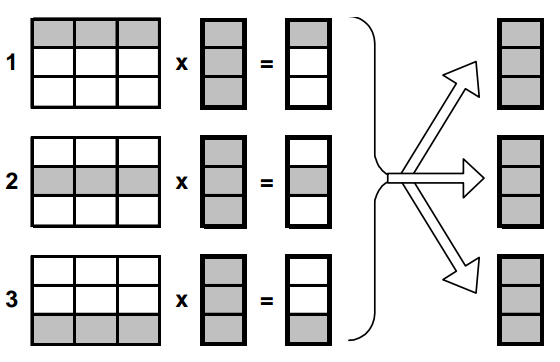
\includegraphics[width=0.75\textwidth]
	{pics/mv_rowwise}
	\caption{Perkalian matriks-vektor Row-Wise Decomposition}
	\label{fig:mv_rowwise}
\end{figure}  

\subsubsection{Column-wise Decomposition}

Algoritma perkalian matriks-vektor ini merupakan alternatif dari \f{row-wise decomposition} di mana pemecahan proses perkalian dilakukan berdasarkan kolom matriks. Setiap proses akan mengalikan sebuah kolom matriks dan sebuah elemen vektor pada satu waktu. Mirip dengan algoritma \f{row-wise decomposition}, jika jumlah prosesor ($np$) lebih sedikit dari jumlah kolom matriks ($c$) maka setiap prosesor bertugas mengalikan $n = \frac{c}{np}$ secara sekuensial.

\begin{figure}
	\centering
	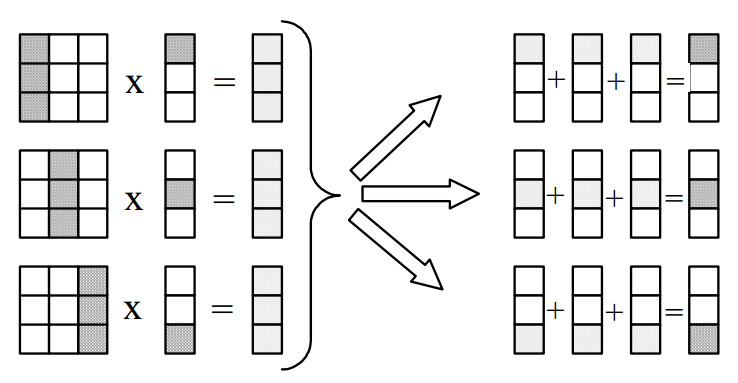
\includegraphics[width=0.9\textwidth]
	{pics/mv_colwise}
	\caption{Perkalian matriks-vektor Column-Wise Decomposition}
	\label{fig:mv_colwise}
\end{figure}  

\subsubsection{Checkerboard Decomposition}

Algoritma perkalian matriks-vektor \f{checkerboard decomposition} ini membagi matriks menjadi submatriks dengan ukuran yang sama dan mengalikannya dengan subvektor yang sesuai. Hasil perkalian tersebut kemudian akan dijumlahkan dan dipetakan ke vektor hasil.

Prekondisi dari algoritma ini adalah jumlah elemen matriks ($n$) harus bisa dibagi rata ke sejumlah prosesor ($np$) atau dengan kata lain memenuhi persamaan \ref{eq:mv_checkerboard}. Hasil pembagian ini ($x$) akan menjadi ukuran submatriks (dan subvektor) yang dikerjakan di tiap proses secara paralel.

\begin{equation}
	x = \sqrt{\frac{n}{np}},\text{ where } x \in \mathbb{Z}
	\label{eq:mv_checkerboard}
\end{equation}


\begin{figure}
	\centering
	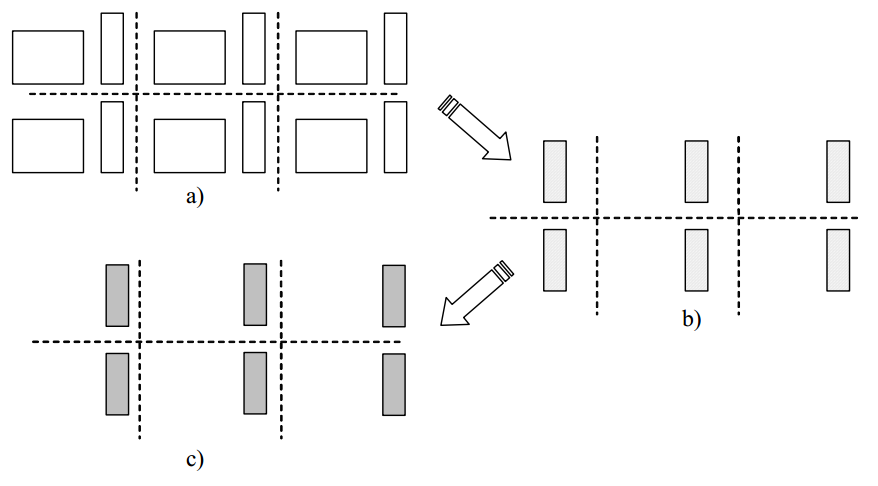
\includegraphics[width=0.75\textwidth]
	{pics/mv_checkerboard}
	\caption{Perkalian matriks-vektor Checkerboard Decomposition}
	\label{fig:mv_checkerboard}
\end{figure}  

\subsection{Perkalian Matriks Bujursangkar} 

\subsubsection{Row-Wise Decomposition}

Mirip dengan algoritma perkalian matriks-vektor \f{row-wise decomposition}, algortima ini juga membagi pekerjaan berdasarkan baris dari matriks pertama seperti yang diilustrasikan pada gambar \ref{fig:mm_rowwise}. Setiap prosesor akan mengalikan sebuah baris dari matriks pertama $A$ dengan seluruh kolom dari matriks kedua $B$. Hasil dari seluruh prosesor kemudian dikonkatenasi menjadi matriks baru $C$.

\begin{figure}
	\centering
	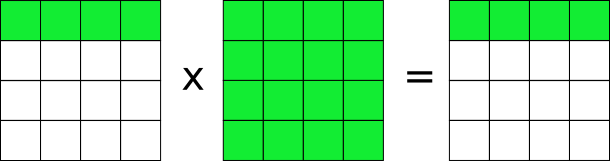
\includegraphics[width=1\textwidth]
	{pics/mm_rowwise}
	\caption{Perkalian matriks bujursangkar Row-Wise Decomposition}
	\label{fig:mm_rowwise}
\end{figure}

\subsubsection{Cannon}

Algoritma Cannon menggunakan dekomposisi seperti algortima matriks-vektor \f{checkerboard decomposition} di mana matriks $A$ dan $B$ dibagi menjadi menjadi submatriks bujursangkar. Perbedaan pada algoritma Cannon adalah prekondisi di mana jumlah proses ($np$) harus merupakan bujursangkar sempurna (\f{perfect square}). Tujuan utama dari algoritma ini adalah untuk meningkatkan efisiensi penggunaan memori pada proses paralel.

\begin{figure}
	\centering
	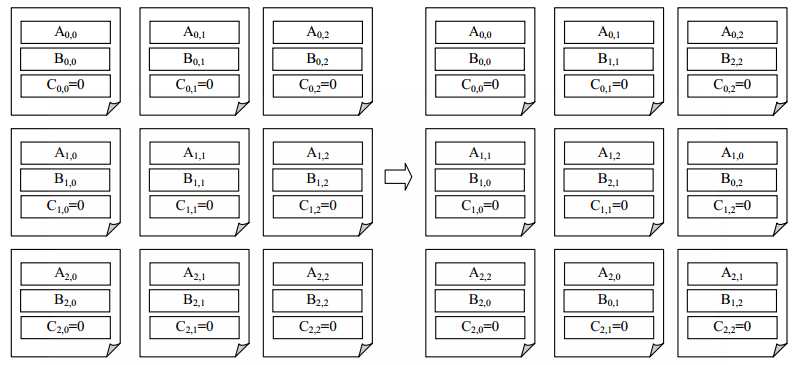
\includegraphics[width=1\textwidth]
	{pics/mm_cannon}
	\caption{Perkalian matriks bujursangkar Cannon}
	\label{fig:mm_cannon}
\end{figure}

\subsubsection{Fox}

Algoritma Fox memiliki kemiripan dengan algoritma Cannon dalam hal dekomposisi matriks menjadi submatriks bujursangkar dan pemetaan prosesor yang harus dapat membentuk bujursangkar sempurna (\f{perfect square}). Yang membedakan algoritma Fox dan Cannon adalah skema distribusi awal submatriks ke prosesor

\begin{figure}
	\centering
	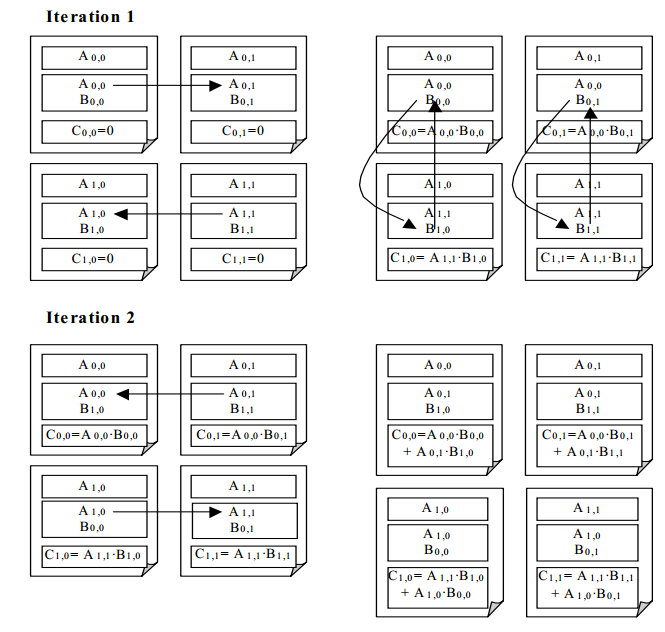
\includegraphics[width=0.75\textwidth]
	{pics/mm_fox}
	\caption{Perkalian matriks bujursangkar Fox}
	\label{fig:mm_fox}
\end{figure}

\subsubsection{DNS}

Algoritma yang diberi nama berdasarkan nama pembuatnya (Dekel, Nassimi and Aahni) ini, diajukan dalam rangka meningkatkan lagi efisiensi penggunaan memori pada perkalian matriks bujursangkar secara paralel. Karakteristik algoritma ini adalah:
\begin{itemize}
	\item Berdasarkan partisi \f{intermediate data}
	\item Melakukan perkalian skalar $n^3$ sehingga membutuhkan proses sebanyak $n \times n \times n$
	\item Membutuhkan waktu komputasi $O(\log n)$ dengan menggunakan $O(\frac{n^3}{\log n})$
\end{itemize}

\begin{figure}
	\centering
	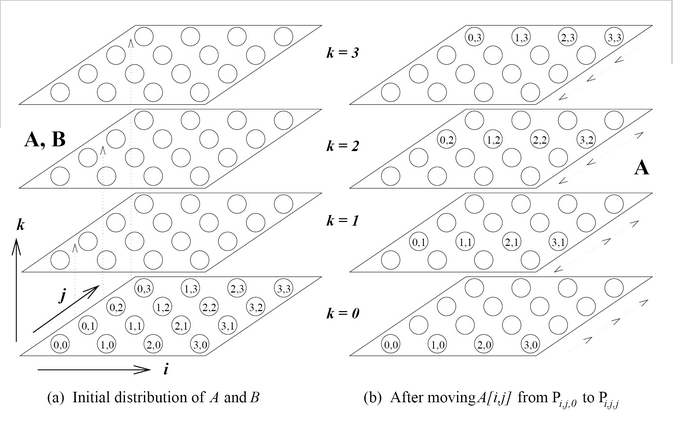
\includegraphics[width=1\textwidth]
	{pics/mm_dns1}
	\caption{Perkalian matriks bujursangkar DNS iterasi 1}
	\label{fig:mm_dns1}
\end{figure}

\begin{figure}
	\centering
	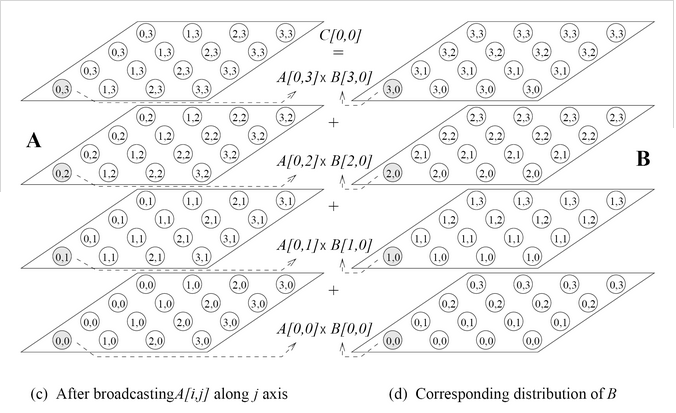
\includegraphics[width=1\textwidth]
	{pics/mm_dns2}
	\caption{Perkalian matriks bujursangkar DNS iterasi 2}
	\label{fig:mm_dns2}
\end{figure}


%-----------------------------------------------------------------------------%
\section{Eksperimen}
%-----------------------------------------------------------------------------%

\subsection{Perkalian Matriks-Vektor} 

\subsubsection{Row-Wise Decomposition}

Algoritma paralel perkalian matriks-vektor yang paling sederhana, yaitu memecah proses perkalian berdasarkan baris matriks (\f{row-wise}). Setiap prosesor akan bertanggung jawab untuk mengalikan sebuah baris matriks dan vektor pada satu waktu. Jika jumlah prosesor ($np$) lebih sedikit dari jumlah baris matriks ($r$) maka setiap prosesor bertugas mengalikan $n = \frac{r}{np}$ secara sekuensial.

\begin{figure}
	\centering
	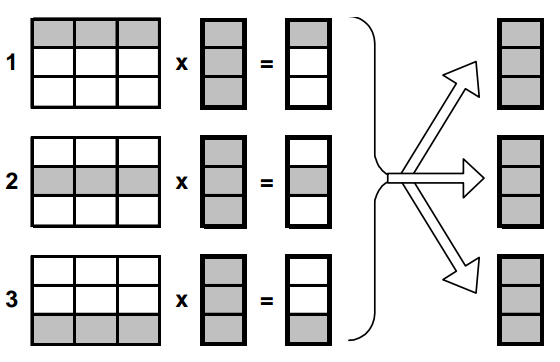
\includegraphics[width=0.75\textwidth]
	{pics/mv_rowwise}
	\caption{Perkalian matriks-vektor Row-Wise Decomposition}
	\label{fig:mv_rowwise}
\end{figure}  

\subsubsection{Column-wise Decomposition}

Algoritma perkalian matriks-vektor ini merupakan alternatif dari \f{row-wise decomposition} di mana pemecahan proses perkalian dilakukan berdasarkan kolom matriks. Setiap proses akan mengalikan sebuah kolom matriks dan sebuah elemen vektor pada satu waktu. Mirip dengan algoritma \f{row-wise decomposition}, jika jumlah prosesor ($np$) lebih sedikit dari jumlah kolom matriks ($c$) maka setiap prosesor bertugas mengalikan $n = \frac{c}{np}$ secara sekuensial.

\begin{figure}
	\centering
	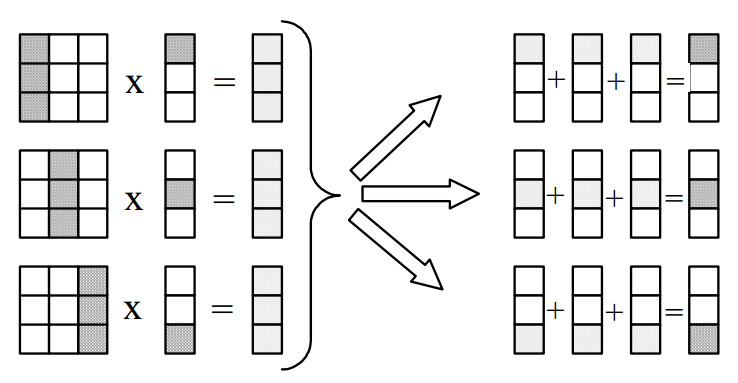
\includegraphics[width=0.9\textwidth]
	{pics/mv_colwise}
	\caption{Perkalian matriks-vektor Column-Wise Decomposition}
	\label{fig:mv_colwise}
\end{figure}  

\subsubsection{Checkerboard Decomposition}

Algoritma perkalian matriks-vektor \f{checkerboard decomposition} ini membagi matriks menjadi submatriks dengan ukuran yang sama dan mengalikannya dengan subvektor yang sesuai. Hasil perkalian tersebut kemudian akan dijumlahkan dan dipetakan ke vektor hasil.

Prekondisi dari algoritma ini adalah jumlah elemen matriks ($n$) harus bisa dibagi rata ke sejumlah prosesor ($np$) atau dengan kata lain memenuhi persamaan \ref{eq:mv_checkerboard}. Hasil pembagian ini ($x$) akan menjadi ukuran submatriks (dan subvektor) yang dikerjakan di tiap proses secara paralel.

\begin{equation}
x = \sqrt{\frac{n}{np}},\text{ where } x \in \mathbb{Z}
\label{eq:mv_checkerboard}
\end{equation}


\begin{figure}
	\centering
	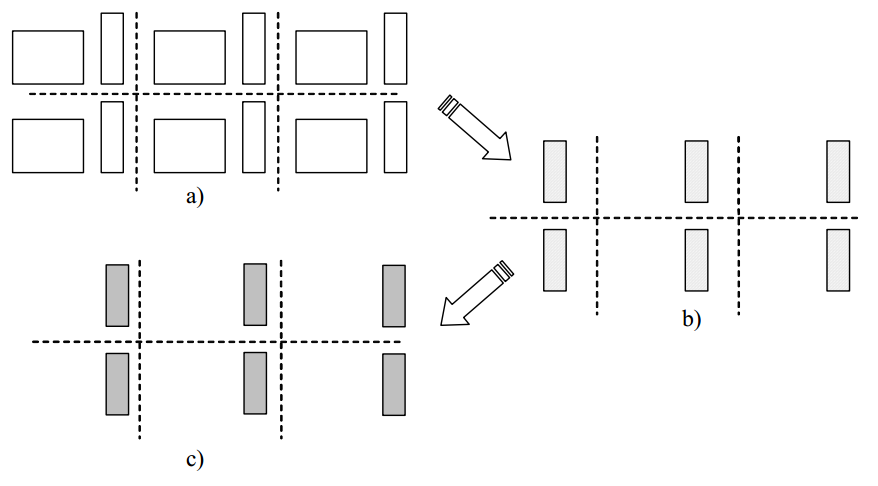
\includegraphics[width=0.75\textwidth]
	{pics/mv_checkerboard}
	\caption{Perkalian matriks-vektor Checkerboard Decomposition}
	\label{fig:mv_checkerboard}
\end{figure}  

\subsection{Perkalian Matriks Bujursangkar} 

\subsubsection{Row-Wise Decomposition}

Mirip dengan algoritma perkalian matriks-vektor \f{row-wise decomposition}, algortima ini juga membagi pekerjaan berdasarkan baris dari matriks pertama seperti yang diilustrasikan pada gambar \ref{fig:mm_rowwise}. Setiap prosesor akan mengalikan sebuah baris dari matriks pertama $A$ dengan seluruh kolom dari matriks kedua $B$. Hasil dari seluruh prosesor kemudian dikonkatenasi menjadi matriks baru $C$.

\begin{figure}
	\centering
	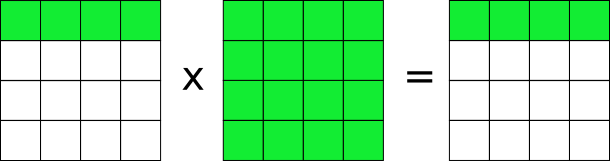
\includegraphics[width=1\textwidth]
	{pics/mm_rowwise}
	\caption{Perkalian matriks bujursangkar Row-Wise Decomposition}
	\label{fig:mm_rowwise}
\end{figure}

\subsubsection{Cannon}

Algoritma Cannon menggunakan dekomposisi seperti algortima matriks-vektor \f{checkerboard decomposition} di mana matriks $A$ dan $B$ dibagi menjadi menjadi submatriks bujursangkar. Perbedaan pada algoritma Cannon adalah prekondisi di mana jumlah proses ($np$) harus merupakan bujursangkar sempurna (\f{perfect square}). Tujuan utama dari algoritma ini adalah untuk meningkatkan efisiensi penggunaan memori pada proses paralel.

\begin{figure}
	\centering
	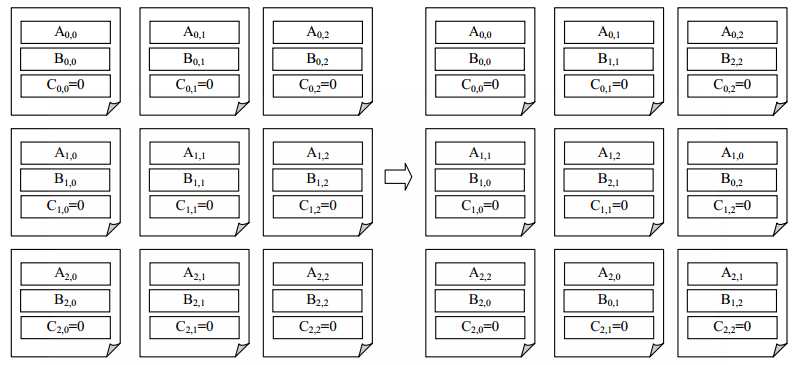
\includegraphics[width=1\textwidth]
	{pics/mm_cannon}
	\caption{Perkalian matriks bujursangkar Cannon}
	\label{fig:mm_cannon}
\end{figure}

\subsubsection{Fox}

Algoritma Fox memiliki kemiripan dengan algoritma Cannon dalam hal dekomposisi matriks menjadi submatriks bujursangkar dan pemetaan prosesor yang harus dapat membentuk bujursangkar sempurna (\f{perfect square}). Yang membedakan algoritma Fox dan Cannon adalah skema distribusi awal submatriks ke prosesor

\begin{figure}
	\centering
	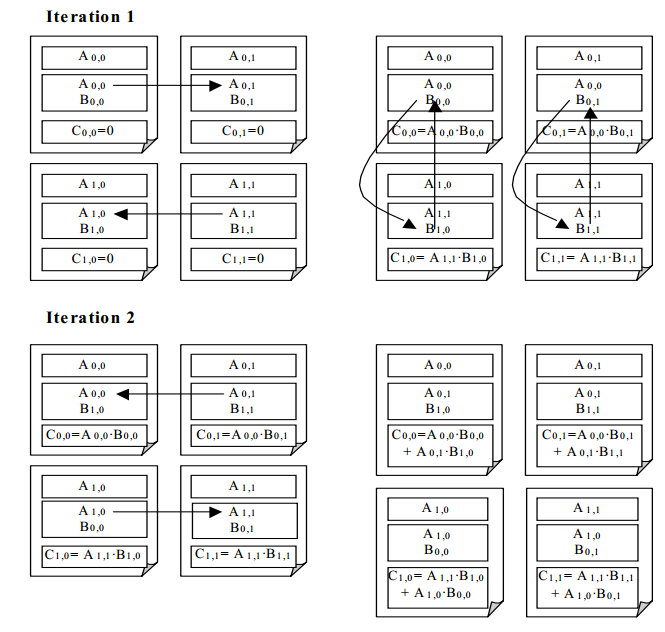
\includegraphics[width=0.75\textwidth]
	{pics/mm_fox}
	\caption{Perkalian matriks bujursangkar Fox}
	\label{fig:mm_fox}
\end{figure}

\subsubsection{DNS}

Algoritma yang diberi nama berdasarkan nama pembuatnya (Dekel, Nassimi and Aahni) ini, diajukan dalam rangka meningkatkan lagi efisiensi penggunaan memori pada perkalian matriks bujursangkar secara paralel. Karakteristik algoritma ini adalah:
\begin{itemize}
	\item Berdasarkan partisi \f{intermediate data}
	\item Melakukan perkalian skalar $n^3$ sehingga membutuhkan proses sebanyak $n \times n \times n$
	\item Membutuhkan waktu komputasi $O(\log n)$ dengan menggunakan $O(\frac{n^3}{\log n})$
\end{itemize}

\begin{figure}
	\centering
	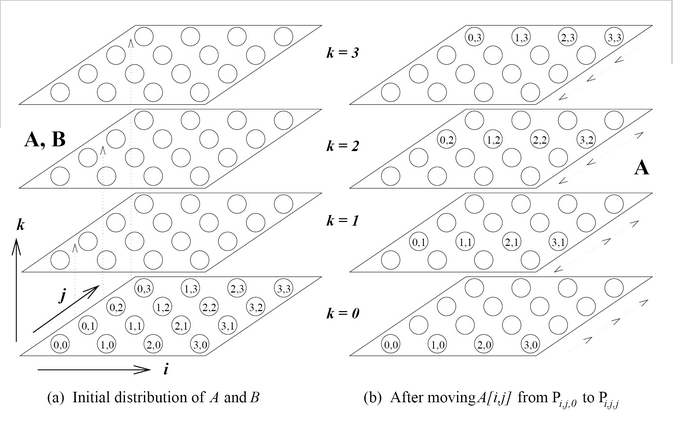
\includegraphics[width=1\textwidth]
	{pics/mm_dns1}
	\caption{Perkalian matriks bujursangkar DNS iterasi 1}
	\label{fig:mm_dns1}
\end{figure}

\begin{figure}
	\centering
	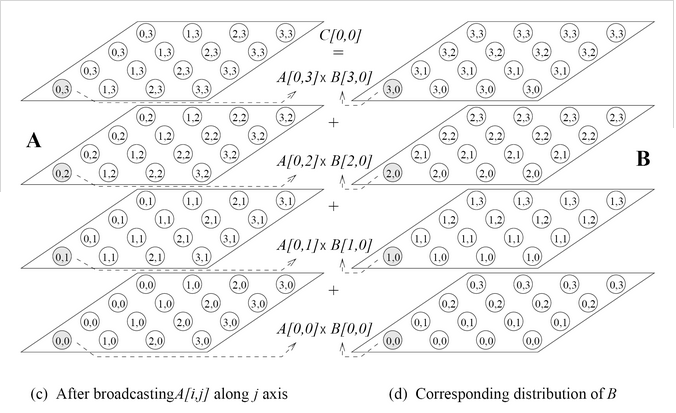
\includegraphics[width=1\textwidth]
	{pics/mm_dns2}
	\caption{Perkalian matriks bujursangkar DNS iterasi 2}
	\label{fig:mm_dns2}
\end{figure}





%-----------------------------------------------------------------------------%
\chapter{\topikDua}
%-----------------------------------------------------------------------------%
\todo{tambahkan kata-kata pengantar bab 2 disini}

%-----------------------------------------------------------------------------%
\section{\latex~Secara Singkat}
%-----------------------------------------------------------------------------%
Berdasarkan \cite{latex.intro}: \\ 
\begin{tabular}{| p{13cm} |}
	\hline 
	\\
	LaTeX is a family of programs designed to produce publication-quality 
	typeset documents. It is particularly strong when working with 
	mathematical symbols. \\	
	The history of LaTeX begins with a program called TEX. In 1978, a 
	computer scientist by the name of Donald Knuth grew frustrated with the 
	mistakes that his publishers made in typesetting his work. He decided 
	to create a typesetting program that everyone could easily use to 
	typeset documents, particularly those that include formulae, and made 
	it freely available. The result is TEX. \\	
	Knuth's product is an immensely powerful program, but one that does 
	focus very much on small details. A mathematician and computer 
	scientist by the name of Leslie Lamport wrote a variant of TEX called 
	LaTeX that focuses on document structure rather than such details. \\
	\\
	\hline
\end{tabular}

\vspace*{0.8cm}

Dokumen \latex~sangat mudah, seperti halnya membuat dokumen teks biasa. Ada 
beberapa perintah yang diawali dengan tanda '\bslash'. 
Seperti perintah \bslash\bslash~yang digunakan untuk memberi baris baru. 
Perintah tersebut juga sama dengan perintah \bslash newline. 
Pada bagian ini akan sedikit dijelaskan cara manipulasi teks dan 
perintah-perintah \latex~yang mungkin akan sering digunakan. 
Jika ingin belajar hal-hal dasar mengenai \latex, silahkan kunjungi: 

\begin{itemize}
	\item \url{http://frodo.elon.edu/tutorial/tutorial/}, atau
	\item \url{http://www.maths.tcd.ie/~dwilkins/LaTeXPrimer/}
\end{itemize}


%-----------------------------------------------------------------------------%
\section{\latex~Kompiler dan IDE}
%-----------------------------------------------------------------------------%
Agar dapat menggunakan \latex~(pada konteks hanya sebagai pengguna), Anda 
tidak perlu banyak tahu mengenai hal-hal didalamnya. 
Seperti halnya pembuatan dokumen secara visual (contohnya Open Office (OO) 
Writer), Anda dapat menggunakan \latex~dengan cara yang sama. 
Orang-orang yang menggunakan \latex~relatif lebih teliti dan terstruktur 
mengenai cara penulisan yang dia gunakan, \latex~memaksa Anda untuk seperti 
itu.  

Kembali pada bahasan utama, untuk mencoba \latex~Anda cukup mendownload 
kompiler dan IDE. Saya menyarankan menggunakan Texlive dan Texmaker. 
Texlive dapat didownload dari \url{http://www.tug.org/texlive/}. 
Sedangkan Texmaker dapat didownload dari 
\url{http://www.xm1math.net/texmaker/}. 
Untuk pertama kali, coba buka berkas thesis.tex dalam template yang Anda miliki 
pada Texmaker. 
Dokumen ini adalah dokumen utama. 
Tekan F6 (PDFLaTeX) dan Texmaker akan mengkompilasi berkas tersebut menjadi 
berkas PDF. 
Jika tidak bisa, pastikan Anda sudah menginstall Texlive. 
Buka berkas tersebut dengan menekan F7. 
Hasilnya adalah sebuah dokumen yang sama seperti dokumen yang Anda baca saat 
ini. 


%-----------------------------------------------------------------------------%
\section{Bold, Italic, dan Underline}
%-----------------------------------------------------------------------------%
Hal pertama yang mungkin ditanyakan adalah bagaimana membuat huruf tercetak 
tebal, miring, atau memiliki garis bawah. 
Pada Texmaker, Anda bisa melakukan hal ini seperti halnya saat mengubah dokumen 
dengan OO Writer. 
Namun jika tetap masih tertarik dengan cara lain, ini dia: 

\begin{itemize}
	\item \bo{Bold} \\
		Gunakan perintah \bslash textbf$\lbrace\rbrace$ atau 
		\bslash bo$\lbrace\rbrace$. 
	\item \f{Italic} \\
		Gunakan perintah \bslash textit$\lbrace\rbrace$ atau 
		\bslash f$\lbrace\rbrace$. 
	\item \underline{Underline} \\
		Gunakan perintah \bslash underline$\lbrace\rbrace$.
	\item $\overline{Overline}$ \\
		Gunakan perintah \bslash overline. 
	\item $^{superscript}$ \\
		Gunakan perintah \bslash $\lbrace\rbrace$. 
	\item $_{subscript}$ \\
		Gunakan perintah \bslash \_$\lbrace\rbrace$. 
\end{itemize}

Perintah \bslash f dan \bslash bo hanya dapat digunakan jika package 
uithesis digunakan. 


%-----------------------------------------------------------------------------%
\section{Memasukan Gambar}
%-----------------------------------------------------------------------------%
Setiap gambar dapat diberikan caption dan diberikan label. Label dapat 
digunakan untuk menunjuk gambar tertentu. 
Jika posisi gambar berubah, maka nomor gambar juga akan diubah secara 
otomatis. 
Begitu juga dengan seluruh referensi yang menunjuk pada gambar tersebut. 
Contoh sederhana adalah \pic~\ref{fig:testGambar}. 
Silahkan lihat code \latex~dengan nama bab2.tex untuk melihat kode lengkapnya. 
Harap diingat bahwa caption untuk gambar selalu terletak dibawah gambar. 

\begin{figure}
	\centering
	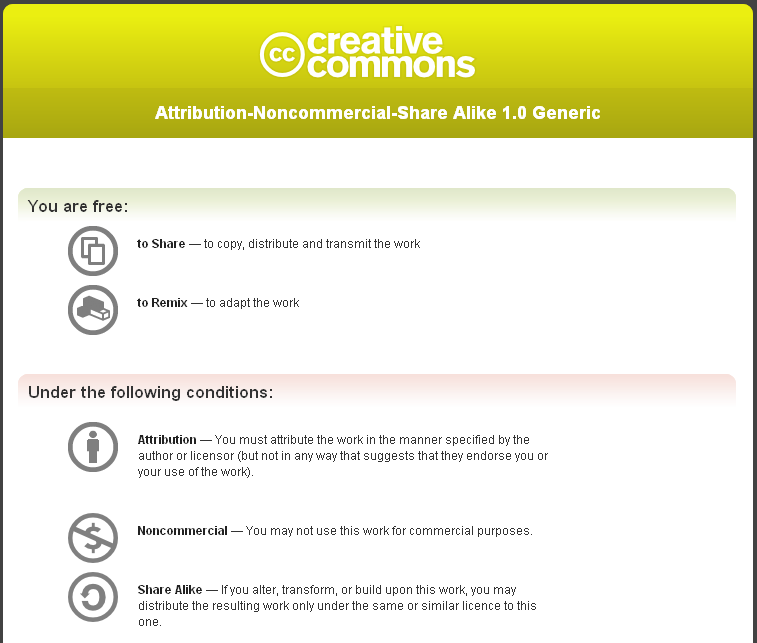
\includegraphics[width=0.50\textwidth]
		{pics/creative_common.png}
	\caption{\license.}
	\label{fig:testGambar}
\end{figure}


%-----------------------------------------------------------------------------%
\section{Membuat Tabel}
%-----------------------------------------------------------------------------%
Seperti pada gambar, tabel juga dapat diberi label dan caption. 
Caption pada tabel terletak pada bagian atas tabel. 
Contoh tabel sederhana dapat dilihat pada \tab~\ref{tab:tab1}.

\begin{table}
	\centering
	\caption{Contoh Tabel}
	\label{tab:tab1}
	\begin{tabular}{| l | c r |}
		\hline
		& kol 1 & kol 2 \\ 
		\hline
		baris 1 & 1 & 2 \\
		baris 2 & 3 & 4 \\
		baris 3 & 5 & 6 \\
		jumlah  & 9 & 12 \\
		\hline
	\end{tabular}
\end{table}

Ada jenis tabel lain yang dapat dibuat dengan \latex~berikut 
beberapa diantaranya. 
Contoh-contoh ini bersumber dari 
\url{http://en.wikibooks.org/wiki/LaTeX/Tables}

\begin{table}
	\centering
	\caption{An Example of Rows Spanning Multiple Columns}
	\label{row.spanning}
	\begin{tabular}{|l|l|*{6}{c|}}
  		\hline % create horizontal line
  		No & Name & \multicolumn{3}{|c|}{Week 1} & \multicolumn{3}{|c|}{Week 2} \\
  		\cline{3-8} % create line from 3rd column till 8th column
  		& & A & B & C & A & B & C\\
  		\hline
  		1 & Lala & 1 & 2 & 3 & 4 & 5 & 6\\
  		2 & Lili & 1 & 2 & 3 & 4 & 5 & 6\\
  		3 & Lulu & 1 & 2 & 3 & 4 & 5 & 6\\
  		\hline
	\end{tabular}
\end{table}

\begin{table}
	\centering
	\caption{An Example of Columns Spanning Multiple Rows}
	\label{column.spanning}
	\begin{tabular}{|l|c|l|}
		\hline
		Percobaan & Iterasi & Waktu \\
		\hline
		Pertama & 1 & 0.1 sec \\ \hline
		\multirow{2}{*}{Kedua} & 1 & 0.1 sec \\
 		& 3 & 0.15 sec \\ 
 		\hline
		\multirow{3}{*}{Ketiga} & 1 & 0.09 sec \\
 		& 2 & 0.16 sec \\
 		& 3 & 0.21 sec \\ 
 		\hline
	\end{tabular}
\end{table}

\begin{table}
	\centering
	\caption{An Example of Spanning in Both Directions Simultaneously}
	\label{mix.spanning}
	\begin{tabular}{cc|c|c|c|c|}
		\cline{3-6}
		& & \multicolumn{4}{|c|}{Title} \\ \cline{3-6}
		& & A & B & C & D \\ \hline
		\multicolumn{1}{|c|}{\multirow{2}{*}{Type}} &
		\multicolumn{1}{|c|}{X} & 1 & 2 & 3 & 4\\ \cline{2-6}
		\multicolumn{1}{|c|}{}                        &
		\multicolumn{1}{|c|}{Y} & 0.5 & 1.0 & 1.5 & 2.0\\ \cline{1-6}
		\multicolumn{1}{|c|}{\multirow{2}{*}{Resource}} &
		\multicolumn{1}{|c|}{I} & 10 & 20 & 30 & 40\\ \cline{2-6}
		\multicolumn{1}{|c|}{}                        &
		\multicolumn{1}{|c|}{J} & 5 & 10 & 15 & 20\\ \cline{1-6}
	\end{tabular}
\end{table}


%---------------------------------------------------------------
\chapter{\kontribusi}
%---------------------------------------------------------------
\todo{Tambahkan kesimpulan dan saran terkait dengan perkerjaan 
	yang dilakukan.}


%---------------------------------------------------------------
\section{Kesimpulan}
%---------------------------------------------------------------


%---------------------------------------------------------------
\section{Saran}
%---------------------------------------------------------------


%
% Daftar Pustaka
%
% Daftar Pustaka 
% 

% 
% Tambahkan pustaka yang digunakan setelah perintah berikut. 
% 
\begin{thebibliography}{4}

\bibitem{opencl.howto}
{Askubuntu.com. \f{How to make OpenCL work on 14.10 + Nvidia 331.89 drivers?}. 10 Oktober 2014. \url{http://askubuntu.com/questions/541114/how-to-make-opencl-work-on-14-10-nvidia-331-89-drivers}.}

\bibitem{opencl.mmul}
{Zaius. \f{Matrix Multiplication 1 (OpenCL)}. 22 September 2009. \url{http://gpgpu-computing4.blogspot.co.id/2009/09/matrix-multiplication-1.html}.}

\bibitem{opencl.mukherjee}
{Mukherjee, S et al. \f{Exploring the Features of OpenCL 2.0}. 2015. IWOCL }

\bibitem{opencl.ebook}
{Banger, R, Bhattacharyya .K. \f{OpenCL Programming by Example}. 2013. Packt publishing }

\bibitem{opencl.clgetplatforminfo}
{Stackoverflow. \f{What is the right way to call clGetPlatformInfo?}. 21 Juni 2013. \url{http://stackoverflow.com/questions/17240071/what-is-the-right-way-to-call-clgetplatforminfo}.}

\bibitem{blas}
{Netlib.org. \f{About BLAS}. 15 November 2015. \url{http://www.netlib.org/blas/​​}.}

\bibitem{opencl.clblas}
{ClMath. \f{ClBLAS}. 2016. \url{https://github.com/clMathLibraries/clBLAS}.}

\bibitem{opencl.clblas.tutorial}
{Nugteren, C. \f{ClBLAS Tutorial}. 2014. \url{http://www.cedricnugteren.nl/tutorial.php?page=1}.}

\bibitem{opencl.mygemm}
{Nugteren, C. \f{MyGEMM}. 2014. \url{https://github.com/cnugteren/myGEMM}.}

\bibitem{opencl.cuda.porting}
{sharcnet.ca. \f{Porting CUDA to OpenCL}. 2014. \url{https://www.sharcnet.ca/help/index.php/Porting_CUDA_to_OpenCL}.}

\bibitem{opencl.mygemm}
{Nugteren, C. \f{Playing with OpenCL: Gaussian Blurring}. 2014. \url{ http://blog.refu.co/?p=663 }.}
​
\end{thebibliography}


%
% Lampiran 
%
%\begin{appendix}
	%%
% @author  Andreas Febrian
% @version 1.00 
% 
% Hanya sebuah pembatas bertuliskan LAMPIRAN ditengah halaman. 
% 

\begin{titlepage}
	\centering 
	\vspace*{6cm}
	\noindent \Huge{LAMPIRAN}
	\addChapter{LAMPIRAN}
\end{titlepage}
	%\setcounter{page}{2}
	%%-----------------------------------------------------------------------------%
\addChapter{Lampiran 1}
\chapter*{Lampiran 1}
%-----------------------------------------------------------------------------%
%\end{appendix}

\end{document}